%%% Erste Seite der Turbulenz %%%
\centering
\section*{\myul{Turbulenz}}

\begin{tikzpicture}[remember picture, overlay]

% --- ERSTE REIHE: Am Seitenursprung anfangen
\setlength{\rowheight}{35mm}

    % A1) Erste Kachel relativ zum Seitenursprung
    \setlength{\cellwidth}{60mm}
    \Tile{A1}{([xshift=10mm, yshift=-20mm]current page.north west)}{\cellwidth}{\rowheight}
        {
            \vspace{-\TileSep}
            \titlebf{Reynoldszahl}\\ \vspace{-3.25mm}
            \begin{equation*}
                \mathrm{Re}_x = \frac{v_\infty\,x}{\nu}
            \end{equation*}
            \rule{\dimexpr\cellwidth-2\TileSep}{0.5pt} \\ \vspace{0.5mm}
            \titlerm{Re\textsubscript{\textit{x},\,krit}}\\ \vspace{-4mm}
            \begin{align*}
                \text{Ebene Platte}&:\text{ 3,5}\cdot 10^5\text{ - 3,2}\cdot 10^6 \\[-0.5ex]
                        \text{Rohr}&:\text{ 2,3}\cdot 10^3\text{ - 4}\cdot 10^4
            \end{align*}
        }{0}{1}{1}{0}

    % B1) Zweite Kachel rechts anbauen
    \setlength{\cellwidth}{65mm}
    \Tile{B1}{(A1.north east)}{\cellwidth}{\rowheight}
        {
            \vspace{-\TileSep}
            \titlebf{Turbulenzgrad (Anströmung)}\\ \vspace{-4mm}
            \begin{equation*}
                \mathrm{Tu} = \frac{1}{\sqrt{3}\,U_\infty}\,\sqrt{\overline{u}'^2 + \overline{v}'^2 + \overline{w}'^2}
            \end{equation*}
            \rule{\dimexpr\cellwidth-2\TileSep}{0.5pt} \\ \vspace{0.5mm}
            \titlebf{Schubspannungsgeschwindigkeit}\\ \vspace{-4mm}
            \begin{equation*}
                u_\tau = \sqrt{\frac{\tau_0}{\rho}}
            \end{equation*}
        }{0}{1}{1}{0}
        
    % C1) Dritte Kachel rechts anbauen
    \setlength{\cellwidth}{65mm}
    \Tile{C1}{(B1.north east)}{\cellwidth}{\rowheight}
        {
            \vspace{-\TileSep}
            \titlebf{e\textsuperscript{\textit{N}}-Methode}\\ \vspace{2mm}
            \begin{equation*}
                \text{e}^N = \exp\!\left(\int_{t_\text{ind}}^{t_\text{krit}} \beta_i\,\text{d}t \right) = \frac{A(x_\text{krit})}{A(x_\text{ind})}
            \end{equation*}
        }{0}{0}{1}{0}

% --- ZWEITE REIHE: Unten anbauen
\setlength{\rowheight}{29mm}

    % A2) Erste Kachel unten anbauen
    \setlength{\cellwidth}{105mm}
    \Tile{A2}{(A1.south west)}{\cellwidth}{\rowheight}
        {
            \titlebf{Reynolds-gemittelte Navier-Stokes-Gleichungen}\\ \vspace{-4mm}
            \begin{align*}
                \rho\,\overline{u}\,\frac{\partial\overline{u}}{\partial x} + \rho\,\overline{v}\,\frac{\partial\overline{u}}{\partial y} &= - \frac{\partial\overline{p}}{\partial x} + \eta\left[\frac{\partial^2\overline{u}}{\partial x^2} + \frac{\partial^2\overline{u}}{\partial y^2}\right] - \rho\,\frac{\partial}{\partial x}\left(\overline{u}'^2\right) - \rho\,\frac{\partial}{\partial y}\left(\overline{u}'\,\overline{v}'\right) \\[0.5ex]
                \rho\,\overline{u}\,\frac{\partial\overline{v}}{\partial x} + \rho\,\overline{v}\,\frac{\partial\overline{v}}{\partial y} &= - \frac{\partial\overline{p}}{\partial y} + \eta\left[\frac{\partial^2\overline{v}}{\partial x^2} + \frac{\partial^2\overline{v}}{\partial y^2}\right] - \rho\,\frac{\partial}{\partial x}\left(\overline{u}'\,\overline{v}'\right) - \rho\,\frac{\partial}{\partial y}\left(\overline{v}'^2\right)
            \end{align*}
        }{0}{1}{1}{0}

    % B2) Zweite Kachel rechts anbauen
    \setlength{\cellwidth}{85mm}
    \Tile{B2}{(A2.north east)}{\cellwidth}{\rowheight}
        {
            \titlebf{Turbulenter Spannungstensor}\\ \vspace{-2mm}
            \begin{equation*}
                \tau_\text{turb} = -\rho\left(
                \begin{matrix}
                    \overline{u}'^2 & \overline{u}'\,\overline{v}' & \overline{u}'\,\overline{w}' \\[1.0ex]
                    \overline{u}'\,\overline{v}' & \overline{u}'^2 & \overline{v}'\,\overline{w}' \\[1.0ex]
                    \overline{u}'\,\overline{w}' & \overline{v}'\,\overline{w}' & \overline{u}'^2
                \end{matrix}
                \right)
            \end{equation*}
        }{0}{0}{1}{0}

% --- DRITTE REIHE: Unten anbauen
\setlength{\rowheight}{20mm}

    % A3) Erste Kachel unten anbauen
    \setlength{\cellwidth}{65mm}
    \Tile{A3}{(A2.south west)}{\cellwidth}{\rowheight}
        {
            \titlebf{Reynoldsspannungen}\\ \vspace{-4.5mm}
            \begin{align*}
                \tau_{xx,\,\text{turb}} &= -\rho\,\overline{u}'^2 \\
                \tau_{yx,\,\text{turb}} &= -\rho\,\overline{u}'\,\overline{v}'
            \end{align*}
        }{0}{1}{1}{0}

    % B3) Zweite Kachel rechts anbauen
    \setlength{\cellwidth}{75mm}
    \Tile{B3}{(A3.north east)}{\cellwidth}{\rowheight}
        {
            \titlebf{Ansatz von Boussinesq}\\ \vspace{-3mm}
            \begin{equation*}
                \tau_\text{ges} = \tau_{yx} + \tau_{yx,\,\text{turb}} = \left(\eta + \eta'\right)\,\frac{\partial\overline{u}}{\partial y}
            \end{equation*}
        }{0}{1}{1}{0}

    % C3) Dritte Kachel rechts anbauen
    \setlength{\cellwidth}{50mm}
    \Tile{C3}{(B3.north east)}{\cellwidth}{\rowheight}
        {
            \titlebf{Scherrate}\\ \vspace{-3.35mm}
            \begin{equation*}
                \frac{\partial\overline{u}}{\partial y} = -\frac{\rho\,\overline{u}'\,\overline{v}'}{\eta'}
            \end{equation*}
        }{0}{0}{1}{0}

% --- VIERTE REIHE: Unten anbauen
\setlength{\rowheight}{44mm}

    % A4) Erste Kachel unten anbauen
    \setlength{\cellwidth}{54mm}
    \Tile{A4}{(A3.south west)}{\cellwidth}{\rowheight}
        {
            \titlebf{Universelles Wandgesetz}\\ \vspace{-4.5mm}
            \begin{equation*}
                u = \frac{\tau_0\,y}{\eta} = \frac{\tau_0\,y}{\rho\,\nu} = \frac{u_\tau^2\,y}{\nu}
            \end{equation*}
            \begin{equation*}
                \Rightarrow\quad\underbrace{\frac{u}{u_\tau}}_{u^{+}} = \underbrace{\frac{u_\tau\,y}{\nu}}_{y^{+}}
            \end{equation*}%
            \vspace{-3mm}
            \begin{align*}
                u^{+} &= \text{Geschwindigkeitsprofil} \\
                y^{+} &= \text{Ausdehnung von Gebiet a}
            \end{align*}
        }{0}{1}{1}{0}

    % B4) Zweite Kachel rechts anbauen
    \setlength{\cellwidth}{74mm}
    \Tile{B4}{(A4.north east)}{\cellwidth}{\rowheight}
        {
            \titlebf{Prandtl'sche Mischungsweghypothese}\\ \vspace{-3mm}
            \begin{equation*}
                \overline{u}'\,\overline{v}' = -l^2\left(\frac{\partial u}{\partial y}\right)\left|\frac{\partial u}{\partial y}\right|
            \end{equation*}
            \rule{\dimexpr\cellwidth-2\TileSep}{0.5pt} \\ \vspace{0.5mm}
            \titlebf{Prandtl'sche Mischungsweglänge}\\ \vspace{-3mm}
            \begin{equation*}
                u' = -l\,\frac{\partial u}{\partial y} = k\,y\,\frac{\partial u}{\partial y} \approx \text{0,41}\,y\,\frac{\partial u}{\partial y}
            \end{equation*}
        }{0}{1}{1}{0}

    % C4) Dritte Kachel rechts anbauen
    \setlength{\cellwidth}{62mm}
    \Tile{C4}{(B4.north east)}{\cellwidth}{\rowheight}
        {
            \titlebf{Logarithmisches Wandgesetz}\\ \vspace{-3.35mm}
            \begin{align*}
                \frac{u}{u_\tau} &= \frac{\ln(10)}{k}\,\log\!\left(\frac{u_\tau\,y}{\nu}\right) + C_2 \\
                                 &\approx \text{5,75}\,\log\!\left(\frac{u_\tau\,y}{\nu}\right) + \text{5,2}
            \end{align*}%
            \vspace{-6mm}
            \rule{\dimexpr\cellwidth-2\TileSep}{0.5pt} \\ \vspace{0.5mm}
            \titlerm{Lokaler Widerstandsbeiwert}\\ \vspace{1mm}
            \begin{minipage}{0.5\cellwidth-\TileSep}
                \centering
                \vspace{-1.5mm}
                \begin{equation*}
                    c_f = \frac{\text{0,370}}{\log(\mathrm{Re}_x)^\text{2,58}}
                \end{equation*}%
                \vspace{-2mm}
            \end{minipage}%
            \vline
            \begin{minipage}{0.5\cellwidth-\TileSep}
                \centering
                \vspace{-1.5mm}
                \begin{equation*}
                    c_\text{W} = \frac{\text{0,455}}{\log(\mathrm{Re}_L)^\text{2,58}}
                \end{equation*}%
                \vspace{-2mm}
            \end{minipage}
        }{0}{0}{1}{0}

% --- FÜNFTE REIHE: Unten anbauen
\setlength{\rowheight}{64mm}

    % A5) Erste Kachel unten anbauen
    \setlength{\cellwidth}{108mm}
    \Tile{A5}{(A4.south west)}{\cellwidth}{\rowheight}
        {
            \titlebf{Gebiete}\\ \vspace{1mm}
            \begin{minipage}{0.48\cellwidth-\TileSep}
                \centering
                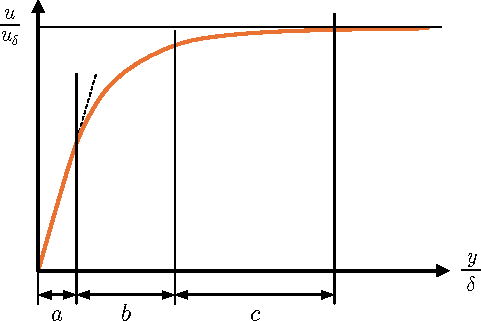
\includegraphics[width=0.94\textwidth]{images/turbulenz-gebiete.pdf}
            \end{minipage}%
            \begin{minipage}{0.52\cellwidth-\TileSep}
                \centering
                \begin{align*}
                    a&:\text{ Laminare Unterschicht (UWG)} \\
                    b&:\text{ Wandnahes Gebiet (LWG)} \\
                    c&:\text{ Außenbereich (PTG)} \\
                \end{align*}
            \end{minipage}%
            \vspace{2mm}
            \rule{\dimexpr\cellwidth-2\TileSep}{0.5pt} \\ \vspace{0.5mm}
            \titlebf{Wandschubspannung}\\ \vspace{1mm}
            \begin{minipage}[t]{0.5\cellwidth-\TileSep}
                \centering
                \titlerm{Platte}\\ \vspace{-4mm}
                \begin{equation*}
                    \tau_0 = \text{0,0225}\,\rho\,u_\infty^2\left(\frac{\nu}{u_\infty\,\delta}\right)^{\frac{1}{4}}
                \end{equation*}
            \end{minipage}%
            \vline
            \begin{minipage}[t]{0.5\cellwidth-\TileSep}
                \centering
                \titlerm{Rohr}\\ \vspace{-4mm}
                \begin{equation*}
                    \tau_0 = \text{0,0225}\,\rho\,u_{\text{max}}^2\left(\frac{\nu}{u_{\text{max}}\,R}\right)^{\frac{1}{4}}
                \end{equation*}%
                \vspace{-2mm}
            \end{minipage}
        }{0}{1}{1}{0}

    % B5) Zweite Kachel rechts anbauen
    \setlength{\cellwidth}{82mm}
    \Tile{B5}{(A5.north east)}{\cellwidth}{\rowheight}
        {
            \titlebf{Potenzgesetz}\\ \vspace{1mm}
            \titlerm{Rohr}\\ \vspace{2mm}
            \begin{minipage}{0.4\cellwidth-\TileSep}
                \centering
                \vspace{-4mm}
                \begin{equation*}
                    \frac{u}{u_\text{max}} = \left(\frac{y}{R}\right)^{\frac{1}{n}}
                \end{equation*}
            \end{minipage}%
            \begin{minipage}{0.6\cellwidth-\TileSep}
                \centering
                \begin{tabular}{c|c|c|c}
                    Re  & $4\cdot 10^3$ & $1\cdot 10^5$ & $2\cdot 10^6$ \\ \hline
                    $n$ & 6             & 7             & 10
                \end{tabular}
            \end{minipage}%
            \vspace{1mm}
            \rule{\dimexpr\cellwidth-2\TileSep}{0.5pt} \\ \vspace{0.5mm}
            \titlerm{Platte}\\ \vspace{1mm}
            \begin{minipage}{0.6\cellwidth-\TileSep}
                \centering
                \vspace{-4mm}
                \begin{equation*}
                    \frac{u}{u_\infty} = \left(\frac{y}{\delta}\right)^{\frac{1}{n}}\qquad n\approx \text{7 - 8}
                \end{equation*}
            \end{minipage}%
            \vline
            \begin{minipage}{0.4\cellwidth-\TileSep}
                \centering
                \myul{Grenzschichtdicke}\\ \vspace{-4mm}
                \begin{equation*}
                    \delta = \frac{\text{0,37}\,x}{\sqrt[5]{\mathrm{Re}_x}} \sim x^{\text{0,8}}
                \end{equation*}%
                \vspace{-2.5mm}
            \end{minipage}%
            \vspace{1.25mm}
            \rule{\dimexpr\cellwidth-2\TileSep}{0.5pt} \\ \vspace{0.5mm}
            \titlerm{Lokaler Widerstandsbeiwert}\\ \vspace{2mm}
            \begin{minipage}{0.5\cellwidth-\TileSep}
                \centering
                \vspace{-1.5mm}
                \begin{equation*}
                    c_f = \frac{\text{0,0576}}{\sqrt[5]{\mathrm{Re}_x}}
                \end{equation*}%
                \vspace{-2mm}
            \end{minipage}%
            \vline
            \begin{minipage}{0.5\cellwidth-\TileSep}
                \centering
                \vspace{-1.5mm}
                \begin{equation*}
                    c_\text{W} = \frac{\text{0,074}}{\sqrt[5]{\mathrm{Re}_L}}
                \end{equation*}%
                \vspace{-2mm}
            \end{minipage}
        }{0}{0}{1}{0}

\end{tikzpicture}

% ### Erste Seite der Fluidkinematik ###
\centering
\vspace{188mm}
\section*{\myul{Fluidkinematik}}

\begin{tikzpicture}[remember picture, overlay]

% --- ERSTE REIHE: Am Seitenursprung anfangen
\setlength{\rowheight}{16mm}

    % X1) Eigene Zeile für die Überschrift
    \Tile{X1}{([xshift=10mm, yshift=-223mm]current page.north west)}{190mm}{8mm}
        {
            \titlebf{Fluidbewegung}
        }{0}{0}{0}{0}

    % A1) Erste Kachel unten anbauen
    \setlength{\cellwidth}{105mm}
    \Tile{A1}{(X1.south west)}{\cellwidth}{\rowheight}
        {
            \vspace{-\TileSep}
            \titlerm{Langrange}\\ \vspace{-3mm}
            \begin{equation*}
                \frac{\text{D} f}{\text{D} t} = \frac{\partial f}{\partial t} + u\,\frac{\partial f}{\partial x} + v\,\frac{\partial f}{\partial y} + w\,\frac{\partial f}{\partial z} = \frac{\partial f}{\partial t} + \underline{v}\cdot\nabla(f)
            \end{equation*}
        }{0}{1}{0}{0}

    % B1) Erste Kachel unten anbauen
    \setlength{\cellwidth}{85mm}
    \Tile{B1}{(A1.north east)}{\cellwidth}{\rowheight}
        {
            \vspace{-\TileSep}
            \titlerm{Euler}\\ \vspace{-3mm}
            \begin{equation*}
                \frac{\text{d} f}{\text{d} t} = \frac{\partial f}{\partial t} + \frac{\partial f}{\partial x}\,\frac{\text{d} x}{\text{d} t} + \frac{\partial f}{\partial y}\,\frac{\text{d} y}{\text{d} t} + \frac{\partial f}{\partial z}\,\frac{\text{d} z}{\text{d} t}
            \end{equation*}
        }{0}{0}{0}{0}

\end{tikzpicture}